\documentclass[10pt]{article}
\usepackage[letterpaper,margin=.6in]{geometry}
\usepackage[T1]{fontenc}
\usepackage{newtxtext,newtxmath,amsmath,graphicx,booktabs,cite,microtype}
\usepackage{float,pdflscape,caption,url}
\usepackage[hidelinks]{hyperref}
\hypersetup{pdftitle={Supplementary Material: Constructive and Destructive Training Regimes},pdfauthor={Thiago Mattar; Cristiano L. Castro; Frederico Coelho; Yan G. Ferreira; Antonio P. Braga}}
\captionsetup{font=small,labelfont=bf}
\renewcommand{\thesection}{S\arabic{section}}
\renewcommand{\thesubsection}{\thesection.\arabic{subsection}}
\renewcommand{\thefigure}{S\arabic{figure}}
\renewcommand{\thetable}{S\arabic{table}}
\renewcommand{\theequation}{S\arabic{equation}}
\newcommand{\E}{\mathbb{E}}
\newcommand{\R}{\mathbb{R}}
\newcommand{\evidence}{../evidence}
\newcommand{\vcassetroot}{../evidence/05-adam/c-intervention}
\title{Supplementary Material\\[3pt]\large Constructive and Destructive Training Regimes:\\From Gradient Interactions to Functional Oscillations}
\author{Thiago Mattar, Cristiano L. Castro, Frederico Coelho, Yan G. Ferreira, Antonio P. Braga}
\date{}
\begin{document}
\maketitle
\noindent This supplement supplies derivations, complete measurement conventions, validation controls, and the full matched intervention grid. Sections S1--S2 support the GD/SGD formulation; S3--S4 support Adam characterization and tracing; S5 supplies intervention methods and outcomes; S6 records reproducibility and scope; S7 retains extended intervention trajectories. Historical MLP replication is explicitly separate from the main one-initialization comparison.
\section{Derivations and the Measurement Clock}

\subsection{State and update indexing}
State $\theta_t$ has $t$ completed updates. The raw gradient $g_t$ is evaluated at that state and is available before the outgoing increment $u_t=\theta_{t+1}-\theta_t$. Paired gradient quantities $\rho_t,r_t,\eta\widehat\kappa_t$ compare states $t-1$ and $t$. Representation motion $\delta_t^\ell=\operatorname{vec}(A_t^\ell-A_{t-1}^\ell)$ is incoming and is displayed at its endpoint $t$. In a fitted window $a{:}b$, the raw-gradient comparison uses $g_{a-1},\ldots,g_{b-1}$, the vectors used for those incoming updates. Earlier source records that number a gradient by the update it supplies are shifted by one when displayed; their numerical values are unchanged.

\subsection{Displacement and directional curvature}
For constant-rate plain SGD, summation gives $\theta_T-\theta_0=-\eta\sum_{t=0}^{T-1}g_t$. Expanding its squared norm gives the main all-pair identity. The triangle inequality gives $0\leq R_T\leq1$ when the total path length is nonzero. For another optimizer, the same geometric identity holds for the actual increments $u_t$, but replacing them by unweighted raw gradients generally does not recover parameter displacement.

For any optimizer, let $u_{t-1}=\theta_t-\theta_{t-1}\ne0$ denote the actual parameter change, and let $f_t=\nabla\mathcal L(\theta_t)$ be the full gradient. For a twice continuously differentiable objective, the fundamental theorem gives
\begin{equation}
 f_t-f_{t-1}=\int_0^1H(\theta_{t-1}+a u_{t-1})u_{t-1}\,da.
\end{equation}
Multiplying by $u_{t-1}^{\top}/\|u_{t-1}\|^2$ proves the step-direction curvature identity in the main text. For sampled gradients $g_t=f_t+\xi_t$, it becomes
\begin{equation}
 \widehat\kappa_t^{\mathrm{step}}
 =\int_0^1\frac{u_{t-1}^{\top}H(\theta_{t-1}+a u_{t-1})u_{t-1}}{\|u_{t-1}\|^2}\,da
 +\frac{u_{t-1}^{\top}(\xi_t-\xi_{t-1})}{\|u_{t-1}\|^2}.
 \label{eq:s-general-curvature}
\end{equation}
The identity does not depend on the choice of optimizer or require the step to be parallel to the gradient. Adam, momentum, clipping, and weight decay may change $u_{t-1}$, but the same formula applies to the actual resulting displacement. For a group-specific learning rate, use the complete applied increment rather than multiplying the entire gradient by one nominal rate.

For full gradients and an $L_H$-Lipschitz Hessian in operator norm along the segment,
\begin{align}
 \left|\widehat\kappa_t^{\mathrm{step}}-
 \frac{u_{t-1}^{\top}H(\theta_{t-1})u_{t-1}}{\|u_{t-1}\|^2}\right|
 &\leq\int_0^1\|H(\theta_{t-1}+a u_{t-1})-H(\theta_{t-1})\|_{\rm op}\,da\notag\\
 &\leq\int_0^1L_Ha\|u_{t-1}\|\,da
 =\tfrac12L_H\|u_{t-1}\|.
\end{align}
This specifies when the measured step-average approximates curvature at its starting point. With sampled gradients, the same bound applies after subtracting the explicit noise term in Eq.~\eqref{eq:s-general-curvature}. Across an activation boundary the smooth assumptions need not hold, even though the gradient-difference diagnostic remains computable.

For plain SGD, $u_{t-1}=-\eta g_{t-1}$ gives
\begin{equation}
 \widehat\kappa_t^{\mathrm{step}}
 =\frac{1}{\eta}\left(1-\frac{g_{t-1}^{\top}g_t}{\|g_{t-1}\|^2}\right)
 =\widehat\kappa_t.
\end{equation}
Its sampling term is $-\varepsilon_t/\eta$, where $\varepsilon_t$ is defined in the main text. In the same specialization the starting-point error bound becomes $L_H\eta\|g_{t-1}\|/2$. For a different optimizer, the raw-gradient combination $\eta\widehat\kappa_t$ and the step-direction curvature are generally different: one projects the gradient change onto the preceding gradient, the other onto the applied increment. The Adam overview retains the former measured quantity and labels it $\eta\widehat\kappa_t$; it is not relabeled as an empirical measurement of the latter.

A zero applied step makes $\widehat\kappa_t^{\mathrm{step}}$ undefined. Separately, $\eta\widehat\kappa_t$ is undefined when $g_{t-1}=0$; if only $g_t=0$, the inner-product expression gives $\eta\widehat\kappa_t=1$ although the gradient cosine is undefined. We use $r_t=\|g_t\|/\|g_{t-1}\|$ as the norm ratio in the supplementary timing tables.

\subsection{Sampling identities and their limits}
Fresh conditional unbiasedness gives $\E[g_{t-1}^\top\xi_t]=0$. At the preceding state, $g_{t-1}=f_{t-1}+\xi_{t-1}$ and $\E[f_{t-1}^\top\xi_{t-1}]=0$, hence
\begin{equation}
 \E[g_{t-1}^\top(\xi_t-\xi_{t-1})]=-\E\|\xi_{t-1}\|^2.
\end{equation}
This reasoning uses conditional expectations before and after the previous sampling decision; it does not assert independence between the new state and the previous noise. For independent uniform batches of $b$ distinct examples from $N$, standard finite-population sampling gives $\operatorname{Cov}(\xi\mid\theta)=(N-b)\Sigma/[b(N-1)]$, where $\Sigma$ uses denominator $N$. Taking its trace yields the variance identity.

At a frozen state, two independent batch gradients satisfy $\E[g^\top g']=\|f\|^2$ and $\E\|g\|^2=\|f\|^2+V_b$. Replacing the product of random norms by $\|f\|^2+V_b$ gives the approximate cosine formula. Neither division of expectations nor replacement of an evolving trajectory by a frozen one is exact. The fixed-state experiment tests these distinctions directly.

\subsection{Finite-step loss and an explicit residual}
Let $x=\theta_{t-1}$, $u=-\eta g_{t-1}$ and $\phi(a)=L(x+a u)$. Then $L_t-L_{t-1}=\int_0^1\phi'(a)\,da$. Integration by parts gives the exact endpoint-trapezoid residual
\begin{equation}
 \mathcal E_t:=L_t-L_{t-1}-\tfrac12(f_{t-1}+f_t)^\top u
 =\int_0^1(\tfrac12-a)u^\top H(x+a u)u\,da.
 \label{eq:t-trapezoid}
\end{equation}
Substituting $f_t=g_t-\xi_t$ yields the main sampled-loss identity. If $H$ is constant, the integral vanishes and full-batch GD gives $\Delta L_t=\eta\|g_{t-1}\|^2(\eta\widehat\kappa_t-2)/2$ exactly. If the Hessian is $L_H$-Lipschitz, subtract its value at the midpoint inside~\eqref{eq:t-trapezoid}; the constant term integrates to zero. Consequently,
\begin{equation}
 |\mathcal E_t|\leq L_H\|u\|^3\int_0^1|a-\tfrac12|^2\,da
 =L_H\|u\|^3/12.
\end{equation}
A small curvature discrepancy does not by itself imply a small error relative to a near-zero loss change. This motivates the separate empirical sign audit. The strict quadratic condition $\eta\widehat\kappa_t>2$ implies $\rho_t<0$ and $r_t>1$, but those two signs alone do not imply it. Current zero gradients and previous zero gradients retain the undefined-case rules in the main text.

\subsection{Adaptive updates}
For full-objective Adam, use $u_t=-\eta_t d_t$, with the parameter-state convention
\begin{align}
 m_t&=\beta_1m_{t-1}+(1-\beta_1)h_t,&
 v_t&=\beta_2v_{t-1}+(1-\beta_2)h_t^{\odot2},\notag\\
 d_t&=\frac{m_t/(1-\beta_1^{t+1})}{\sqrt{v_t/(1-\beta_2^{t+1})}+\epsilon},&
 \theta_{t+1}&=\theta_t-\eta_t d_t.
\end{align}
Moments are initialized to zero at index $-1$. Here $h_t=g_t$ for native Adam and $h_t=\min(1,\gamma/\|g_t\|)g_t$ for global clipping, with factor one when $g_t=0$. The raw diagnostic always uses the unclipped $g_t$. Late $\beta_2$ interventions preserve moments and the native counter; their bias correction uses the new coefficient and that existing counter, rather than a product of historical coefficients. Caps subsequently transform the stored parameter proposal while retaining these advanced moments. The step-direction estimate uses the actual increment after any intervention. The raw-gradient quantity $\eta\widehat\kappa_t$ continues to describe gradient reversal and growth, with the distinct interpretation explained above.

\section{GD/SGD Methods and Independent Checks}

\subsection{Objectives, data preparation, and numerical conventions}
The MLP has dimensions 3072--200--200--10 with tanh hidden activations, 656,810 parameters, and half-squared error summed over the ten outputs and averaged over the first 5,000 CIFAR-10 training images. Standardization uses coordinate-wise statistics from the complete training split. ResNet-32 uses all 50,000 training images, channel-wise training-split standardization, and mean cross-entropy with 50 fixed groups of 1,000 images for BatchNorm. Group composition is preserved during gradient accumulation and probing; normalization is a part of the fixed objective, not silently changed to inference-mode statistics. There is no data augmentation or dropout.

The two-layer, two-head word-level Transformer has embedding and feed-forward widths 200. Twenty corpus streams form causal chunks of at most 35 tokens: 59,680 prepared sequences with 2,088,600 supervised targets. Loss sums valid-token negative log likelihood and divides by the complete target count, excluding padding. The 33,278-word first-occurrence dictionary over training, validation, and test text follows the pinned PyTorch example revision \texttt{13acec6d7c78}~\cite{pytorchWordLanguageModelPinned}. This is a fixed-objective dynamics setup, not a train-only-vocabulary benchmark. Held-out words enter dictionary construction, but held-out losses are not used for updates or intervention selection.

Parameters, stored gradients, and moments are FP32; diagnostic products and norms are reduced in FP64. TF32 is disabled. Spectra use the largest algebraic Hessian eigenvalue at steps $0,100,\ldots,3000$, with relative eigenpair residual at most $.005$. MLP spectral coverage is complete; ResNet uses five intact normalization groups and Transformer uses 2,500 sequences. In main Fig. 1, sparse spectra are interpolated before the same centered 101-step mean used for $Q_s$; no additional Hessian observation is created. Main Fig. 2 uses complete trailing 50-observation means for norms/cosines and raw prefix $R_s$.

\begin{table}[H]
\centering\small
\caption{Complete GD endpoint and finite-step sign audit. $E=\sum\|g_s\|^2$, $I_{\rm all}=2\sum_{i<j}g_i^\top g_j$, and $I_1=2\sum_s g_{s-1}^\top g_s$ use all applied gradients. Ratios remove the common $\eta^2$ factor. Sign errors compare the incoming quadratic surrogate with 2,999 actual transitions; the final unpaired update is excluded. No noise is present.}
\label{tab:s-gd}
\begin{tabular}{llrrrrr}
\toprule
Model & $\eta$ & $L_{3000}$ & $R_{3000}$ & $I_{\rm all}/E$ & $I_1/E$ & Sign errors \\
\midrule
MLP & 0.004 & 0.3365 & 0.7941 & 847.349 & 1.905 & 0/2999 \\
MLP & 0.02 & 0.2114 & 0.0488 & 2.988 & -1.970 & 145/2999 \\
MLP & 0.04 & 0.1539 & 0.0257 & 0.659 & -1.945 & 281/2999 \\
ResNet-32 & 0.025 & 1.4665 & 0.1385 & 37.798 & -1.884 & 595/2999 \\
ResNet-32 & 0.05 & 0.9672 & 0.0616 & 7.375 & -1.900 & 694/2999 \\
ResNet-32 & 0.1 & 0.4898 & 0.0374 & 2.427 & -1.900 & 814/2999 \\
Transformer & 0.05 & 6.6301 & 0.7223 & 620.733 & 1.977 & 0/2999 \\
Transformer & 0.1 & 6.3519 & 0.1395 & 50.112 & -1.631 & 542/2999 \\
Transformer & 0.2 & 6.0697 & 0.0541 & 7.671 & -1.927 & 1325/2999 \\
\bottomrule
\end{tabular}

\end{table}

All nine total interaction ratios are positive, whereas seven adjacent ratios are negative. These are exact sum reductions of finite trajectories, not estimates with independent-update confidence intervals. The backward-lag profiles use separate qualified continuations from step 2,000 and a fixed endpoint at 2,256. Floating-point trajectories can differ from the original long GD run; the displayed lag profile is not silently spliced into its all-pair accounting.

\subsection{Sampling design and dependence}
MLP batch sizes are 32/128/512/2048/5000 images; ResNet sizes are 1/5/20/50 complete normalization groups; Transformer sizes are 8/32/128/512/59680 sequences. Batches are independently redrawn uniform subsets without replacement. Within a repetition, different sizes use prefixes of a common permutation. For Transformer sequence-summed losses $\ell_i$, the estimator is $N(bM)^{-1}\sum_{i\in B}\ell_i$, with $N=59680$ and $M=2088600$. Its fixed denominator preserves unbiasedness for the full token-weighted objective; dividing by the random sampled token count would define a different estimator.

Each of three initializations supplies new matched GD reference states. The main two-start comparison uses states 0/2000, 200 updates, eight stochastic repetitions per cell, and one deterministic full-GD continuation per initialization/start. It comprises 546 continuations. MLP additionally has a state-1000 calibration block. Its historical initialization-0 reconstruction did not pass the specified scalar tolerance, so the sampling study uses new matched references instead of claiming exact recovery of that earlier path. Corresponding native full-GD continuation segments were checked against their own references.

The smallest two ResNet batches in initialization 2 use a different runtime. A 200-update full-GD bridge has parameter relative error $2.36\times10^{-7}$, but batch and runtime remain confounded in that block. Means and ranges across three initialization blocks describe that combined variability. Equal update counts imply different data exposure; neither convergence speed per example nor a wall-time advantage is inferred.

\subsection{Frozen sampling and directional HVP validation}
At nine MLP reference states (three initializations, steps 0/1000/2000), each batch-size cell has 32 independent sequences of 128 frozen draws. The 184,320 total observations include deterministic full-batch controls. Figure~\ref{fig:s-frozen} compares exact moment targets and the approximate expected cosine. Conditional 95\% intervals use 4,000 sequence-bootstrap resamples; they are not seed-level confidence intervals.

\begin{figure}[H]
\centering
\includegraphics[width=7.16in]{\evidence/04-gd-sgd/support/frozen_calibration.pdf}
\caption{Frozen-state MLP calibration. Each point is one saved-state/batch condition; color identifies batch and marker identifies state. Moment quantities share the normalization $\|f\|^2+V_b$; cosine is compared with $\|f\|^2/(\|f\|^2+V_b)$. Bars are conditional 95\% sequence-bootstrap intervals. Parameters never change. Maximum relative moment discrepancies are $.50\%/ .74\%$; maximum absolute cosine error is $.00745$, with 21/36 stochastic intervals missing the approximation.}
\label{fig:s-frozen}
\end{figure}

The separate moving MLP experiment contains 297 continuations across the three starts and five batch sizes. Four state-matched derivative pairs per continuation produce 1,188 comparisons. Each reference evaluates a directional HVP of the complete objective at the starting state; full gradients at both states supply the realized noise difference. Table~\ref{tab:s-hvp} compares $Q_s$ and $Q_s+\varepsilon_s$ with the independent scaled Rayleigh quotient. The correction is algebraic, but the HVP is separately computed. Measurements are dependent within trajectories.

\begin{table}[H]
\centering\small
\caption{Absolute discrepancy from the independently computed scaled directional HVP. Medians and 90th percentiles are over raw paired observations, not smoothed curves. Full-gradient references make correction an offline validation.}
\label{tab:s-hvp}
\input{\evidence/04-gd-sgd/tables/analysis027_hvp_errors.tex}
\end{table}

\begin{figure}[H]
\centering
\includegraphics[width=7.16in]{\evidence/04-gd-sgd/support/sgd_proxy_validation.pdf}
\caption{Directional-curvature validation in the tanh MLP. Raw paired markers compare the two-gradient response, its realized-noise correction, and independently measured directional HVPs. Smoothed trajectories supply context only. The complete objective covers all 5,000 examples; this is neither a largest-eigenvalue comparison nor a validated online noise estimator.}
\end{figure}

\clearpage
\section{Adam Timing, Severity, and Warning Memory}

\subsection{Trajectories, event selection, and targets}
The complete comparison has nine full-objective Adam trajectories: MLP rates $.0001/.0003/.001$ and ResNet/Transformer rates $.0003/.001/.003$, each for 1,024 updates with one initialization per model. Initial tensors agree across rates within a model, moments start at zero, and the native coefficients are $(.9,.999)$ with $\epsilon=10^{-8}$ and no clipping, decay, or schedule. Numerical runtimes differ across some arms; hardware effects are not separately randomized.

A loss excursion starts at a strict increase, fixes the preceding state as its baseline, and tracks the peak until the first return to or below that baseline. An excursion still open at the horizon is right-censored. The overview uses a zero-based vertical range for $\eta\widehat\kappa_t$, leaving 13/17/1 negative MLP/ResNet/Transformer values outside view without changing them. Overview shading uses baseline-to-peak intervals whose maximum exceeds baseline by more than 10\%; outlined intervals retain unobserved recovery. These event definitions are distinct from the individual-step targets used below. A sequence of upward updates is not a sequence of independent spikes.

Decisions at $t=1,\ldots,1023$ use only available raw-gradient information. At future offset $h$, the individual target is
\begin{equation}
 Y_{t,h}(\delta)=\mathbf1\{(L_{t+h}-L_{t+h-1})/L_{t+h-1}\geq\delta\},
\end{equation}
with strict positivity for the zero-threshold case. Net targets instead compare $L_{t+h}$ with $L_t$; within-horizon targets compare $\max_{1\leq j\leq h}L_{t+j}$ with $L_t$. The common cohort $t=1,\ldots,1008$ supports all $h=1,\ldots,16$ without changing endpoint composition. A second analysis restricts decisions to $L_t\leq L_{t-1}$; it excludes an already-rising step, not necessarily an ongoing excursion.

Coverage is $\mathrm{TP}/(\mathrm{TP}+\mathrm{FN})$, precision is $\mathrm{TP}/(\mathrm{TP}+\mathrm{FP})$, and the false-positive rate is $\mathrm{FP}/(\mathrm{FP}+\mathrm{TN})$. Precision lift uses the unconditional target frequency in the identical cohort. Undefined ratios remain missing. The flags $D=(\rho_t<0)$, $G=(r_t>1)$, $D\wedge G$, and $\eta\widehat\kappa_t\geq2$ are evaluated before the outgoing update. The angle/norm form of $\eta\widehat\kappa_t>2$ is algebraically equivalent, not a fifth signal.

\begin{table}[H]
\centering\small
\caption{Complete next-step sign accounting in the three displayed high-rate arms. Each signal cell gives flagged increases/flagged decreases; target totals are in the second and third columns. The upper block concerns strictly positive or negative individual changes. The lower block gives confusion counts for the main 0.1\% next-step target, using the same 1,023 decisions; non-target steps include smaller rises. Neither target counts recovered excursions.}
\begin{tabular}{@{}lrrrrrr@{}}
\toprule
Case & Increases & Decreases & $D$ up/down & $G$ up/down & Both up/down & $\eta\widehat\kappa\geq2$ up/down \\
\midrule
MLP & 454 & 569 & 404/412 & 261/285 & 239/218 & 172/136 \\
ResNet & 95 & 928 & 86/214 & 47/277 & 46/116 & 21/15 \\
Transformer & 152 & 871 & 145/376 & 99/322 & 98/203 & 81/66 \\
\bottomrule
\end{tabular}
\medskip
\begin{tabular}{@{}lrrr@{}}
\toprule
0.1\% target: TP / FP / FN / TN & MLP & ResNet & Transformer \\
\midrule
$L_t>L_{t-1}$ & 236/219/210/358 & 35/60/53/875 & 78/74/64/807 \\
$\rho_t<0$ & 398/418/48/159 & 81/219/7/716 & 135/386/7/495 \\
$\|g_t\|>\|g_{t-1}\|$ & 258/288/188/289 & 46/278/42/657 & 93/328/49/553 \\
$\eta\widehat\kappa_t\geq2$ & 172/136/274/441 & 21/15/67/920 & 79/68/63/813 \\
\bottomrule
\end{tabular}
\end{table}

For the main 0.1\% target, the event totals are 446/88/142. Classification accuracy is $(\mathrm{TP}+\mathrm{TN})/1023$. Warning hit rate is precision, and its lift uses the event frequency above. The naive history rule flags any strictly positive preceding change; it does not inspect the next loss. Strict angle/norm and non-strict projected-response thresholds agree here because no measured value equals two. The table exposes the false alarms and misses behind the main comparison.

Warning memory flags a decision if a condition occurred at any of the last $w$ states, including the current one. All $w=1,\ldots,16$ use $t=16,\ldots,1023$, and each target update is counted once. Enlarging the memory window enlarges the flag set; improved coverage must be assessed with its additional false alarms. Similarly, a longer future search window increases the opportunity for a positive target.

These grids are exploratory characterization on previously inspected trajectories. Thresholds, horizons, and selected high-rate displays do not constitute prospective confirmation. Temporal dependence and one initialization per model preclude independent-seed confidence intervals. A validated predictor would require fixed targets and horizons, temporal separation, loss-history and norm baselines, and fresh-seed evaluation.

Across all nine rates, 9,207 eligible decisions contain 2,233 increases and 6,974 decreases. The $\eta\widehat\kappa_t\geq2$ condition covers 853 increases and flags 955 decreases. On the common 1,008-state high-rate cohort, Transformer coverage of individual increases of at least 10\% is 22/26, 25/26, and 26/26 at offsets one, two, and three. At offset three, precision is 26/147 (17.7\%) against a target frequency of 26/1008 (2.6\%). All three MLP increases of at least 50\% evade the current $\eta\widehat\kappa_t$ condition. Retaining a condition for 16 states covers every next-step rise of at least 10\% on its common cohort, while flagging 688/248/488 non-target steps. These are descriptive comparisons of overlapping decisions, not independent events or a validated choice of horizon.

\clearpage
\begin{landscape}
\begin{figure}[H]
\centering
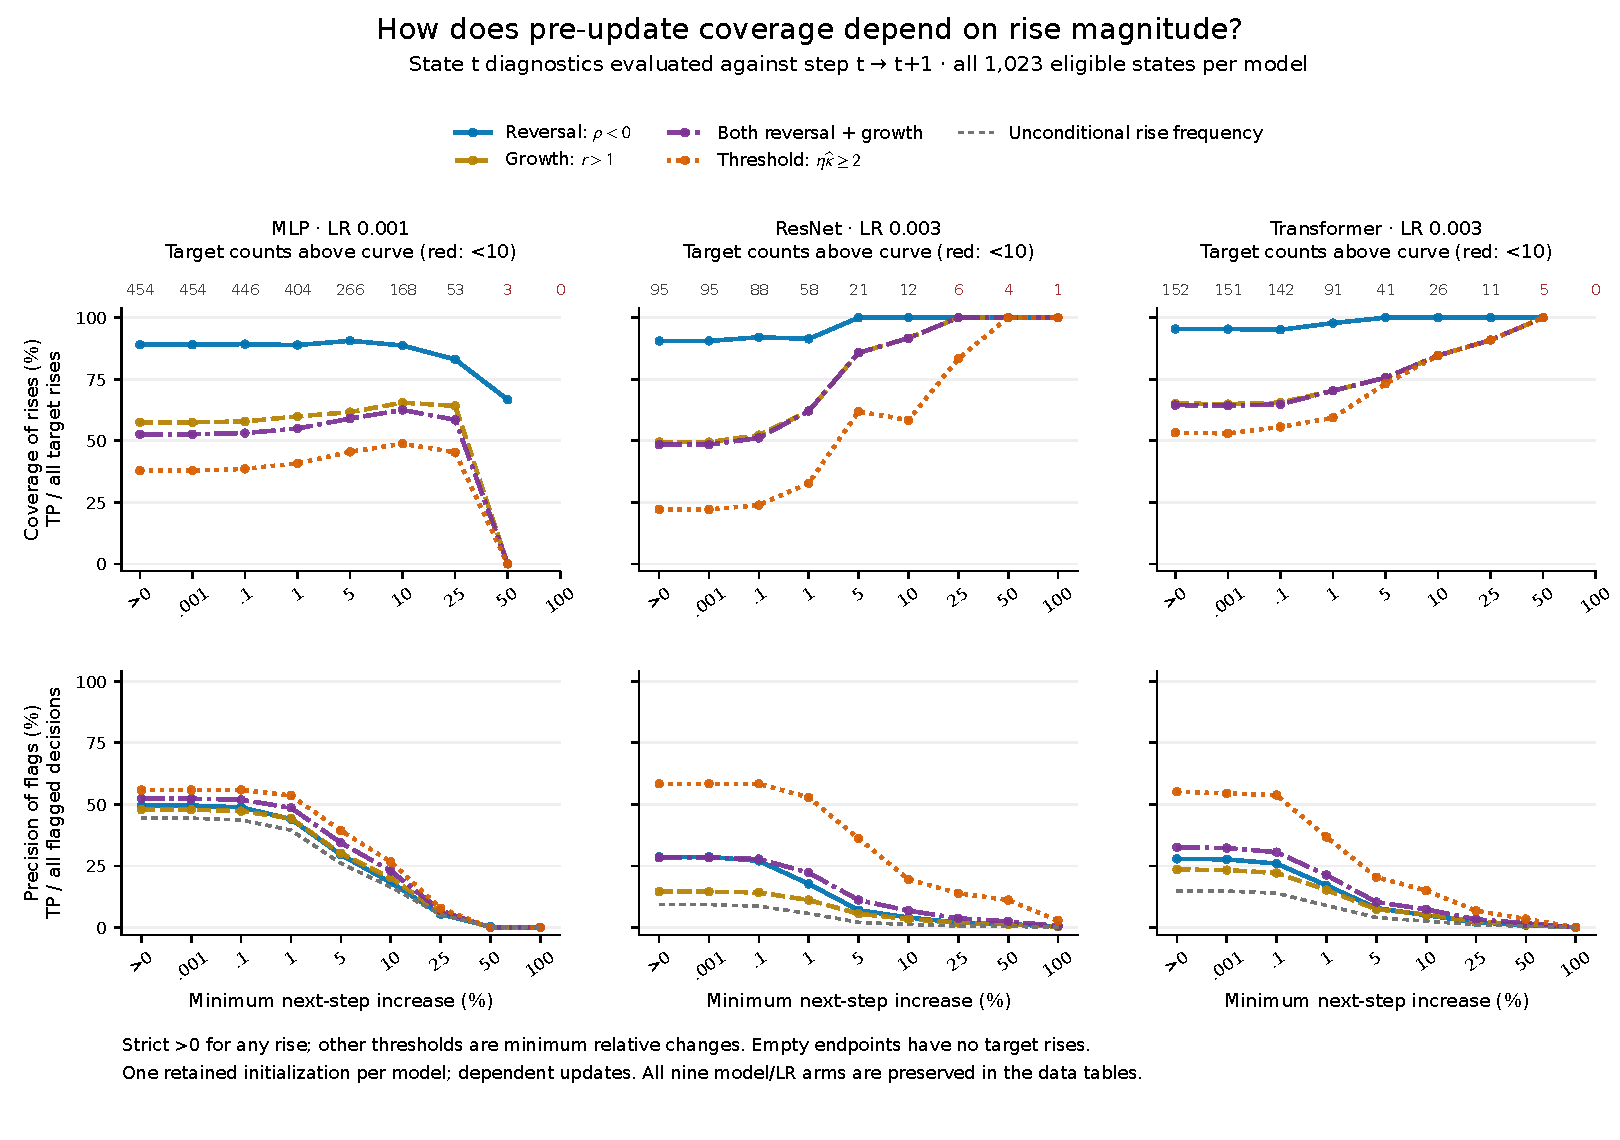
\includegraphics[page=1,width=9.6in]{figures/adam_forward_and_severity.pdf}
\caption{Coverage and precision versus minimum next-step relative loss increase. All 1,023 eligible decisions per model are retained; counts identify rare targets. Reversal, growth, their conjunction, and the projected-response threshold are compared with unconditional frequency.}
\end{figure}
\end{landscape}
\clearpage
\begin{landscape}
\begin{figure}[H]
\centering
\includegraphics[page=2,width=9.6in]{figures/adam_forward_and_severity.pdf}
\caption{Individual loss increases of at least 10 percent at each future offset. All offsets use the same 1,008 decision states. Coverage and precision describe the current flag at that offset; they are not validation of an outcome-selected lead time.}
\end{figure}
\end{landscape}
\clearpage
\begin{landscape}
\begin{figure}[H]
\centering
\includegraphics[page=3,width=9.6in]{figures/adam_forward_and_severity.pdf}
\caption{Net loss increase of at least 10 percent from the decision state to each future horizon. This target differs from an individual future step increase; common decision support is retained.}
\end{figure}
\end{landscape}
\clearpage
\begin{landscape}
\begin{figure}[H]
\centering
\includegraphics[page=4,width=9.6in]{figures/adam_forward_and_severity.pdf}
\caption{Any loss at least 10 percent above the decision-state loss within the future horizon. The target set expands with the horizon, so increasing precision must be compared with its rising base frequency.}
\end{figure}
\end{landscape}
\clearpage
\begin{landscape}
\begin{figure}[H]
\centering
\includegraphics[page=5,width=9.6in]{figures/adam_forward_and_severity.pdf}
\caption{Within-horizon increases restricted to currently non-rising decisions. This excludes an already-rising step but not necessarily an ongoing excursion. Sparse threshold support and target frequencies remain visible.}
\end{figure}
\end{landscape}
\clearpage
\begin{landscape}
\begin{figure}[H]
\centering
\includegraphics[page=6,width=9.6in]{figures/adam_forward_and_severity.pdf}
\caption{Remembered warnings for the unique next-step target. Each target is counted once; all memory widths use decisions 16--1023. Longer memory increases both coverage and the number of non-target flags.}
\end{figure}
\end{landscape}


\clearpage
\section{Representation Tracing: Coordinates, Controls, and Coverage}

\subsection{Fixed inputs and observer qualification}
Each reference set fixes input identities, order, context, masks, and coordinate correspondence across parameter states. Flattening an activation tensor retains every sample/token/spatial/feature entry. The cosine therefore compares changes on multiple \emph{matching} inputs, not averaged representations. The MLP reference set covers all 5,000 training images. ResNet uses the first intact original 1,000-image training-mode BatchNorm group. Transformer uses the first 64 prepared sequences and all 2,240 supervised positions. These latter reference sets are convenient fixed subsets, without replication across independently chosen reference sets or a claim of population-wide activation representativeness.

The observer preserves original model modes, RNG, buffers, normalization groups, and gradients. Identical-state repeat and plain-forward checks establish observer invariance in these deterministic settings. Training gradients still use the complete objective. The selected ResNet trace is the qualified native continuation around the 415 peak: all 187 loss states from 264 through 450 reproduce exactly, with initial gradient and state-296 parameter/gradient audit agreement. All six displayed site cosine/RMS histories agree with the paired motion figure. This qualifies that continuation; it is not bitwise recovery of a different runtime's original overview trajectory.

The measured endpoints are: MLP first linear map, first tanh, second linear map, second tanh, and output; ResNet first convolution, residual block groups 1/2/3, pooling, and output log probabilities; Transformer embedding, attention output and block output in each of two layers, and output log probabilities. These are computational boundaries, not averages over every internal operation. In particular, an attention-output trace does not separately identify query, key, value, and attention-weight mechanisms.

\subsection{Output spaces and loss relevance}
The MLP uses raw outputs, matching its half-squared error. ResNet and Transformer use all-class/all-vocabulary log probabilities, removing the softmax invariance to a common logit shift. Their Euclidean geometry still gives all coordinates equal weight; it is not automatically a loss-sensitivity metric. A correct-label log-probability readout has negative mean equal to the reference-set cross-entropy under the stated image/token weighting. This checks the loss readout without replacing the full output tensor in the primary SVD.

\subsection{Temporal reduction and descriptive controls}
Primary windows contain incoming changes at completed steps 451--501, 390--450, and 553--601, giving 51/61/49 rows. The extra predecessor used for the first cosine is excluded from the fitted matrix. The temporal Gram is accumulated in FP64 over coordinate blocks without example averaging, centering, random projection, or primary row normalization. Numerical PSD, trace, eigenvalue, and coefficient reconstruction checks qualify the reduction. Spatial patterns remain fixed over the fitted window; this does not imply that local dominant directions cannot rotate within their span.

For temporal Gram $K$, the orthogonal reference $K_{\rm orth}=\operatorname{diag}(\operatorname{diag}K)$ keeps all individual step norms and removes directional cross-terms. Unit-row normalization uses $K_{\rm unit}=B^{-1/2}KB^{-1/2}$ with $B=\operatorname{diag}(\operatorname{diag}K)$, excluding zero rows. Table~\ref{tab:t-spectral} separates amplitude weighting from directional structure. These references are not randomized significance tests. Since $PKP^\top$ has the same eigenvalues for every temporal permutation $P$, spectral concentration alone cannot establish oscillation; the signed coefficient series supplies temporal order.

\begin{table}[H]
\centering\small
\caption{Output-change spectral controls. $r_{95}$ is the number of modes needed for 95\% energy; $T$ is the fitted row count. Primary, orthogonal, and unit-row results use the same selected window.}
\label{tab:t-spectral}
\setlength{\tabcolsep}{6pt}
\begin{tabular}{@{}lr rr rr rr@{}}
\toprule
 & & \multicolumn{2}{c}{Observed} & \multicolumn{2}{c}{Same norms, orthogonal} & \multicolumn{2}{c}{Unit rows} \\
Case & $T$ & Top 1 (\%) & $r_{95}$ & Top 1 (\%) & $r_{95}$ & Top 1 (\%) & $r_{95}$ \\
\midrule
MLP & 51 & 53.02 & 5 & 7.85 & 42 & 36.21 & 5 \\
ResNet & 61 & 27.26 & 20 & 9.95 & 31 & 10.85 & 33 \\
Transformer & 49 & 41.65 & 15 & 16.72 & 20 & 16.77 & 29 \\
\bottomrule
\end{tabular}
\end{table}

Reference sets and windows differ across models; these are descriptive within-window measurements, rather than a controlled comparison of architecture dimensionality or causal propagation.

\subsection{Representation displacement retention}
For the same incoming changes $a{:}b$, let $K_\ell=D_\ell D_\ell^\top$.
Without truncating its modes, $R_{a:b}^\ell=\sqrt{\mathbf1^\top K_\ell\mathbf1}/\sum_i\sqrt{(K_\ell)_{ii}}$.
The direct Gram sum and full eigendecomposition agree numerically. Output values are
$.0170537/.0243649/.0350844$ for MLP/ResNet/Transformer; their first measured
sites give $.0325244/.0372071/.2433357$. The windows contain 51/61/49 changes.
A zero path length leaves retention undefined. Low retention alone need not
imply reversal: equal-length orthogonal changes yield $1/\sqrt{T_w}$.

\clearpage
\section{Matched Interventions and Complete Outcomes}

\subsection{Input geometry and what the cap bounds}
Write the native proposal for one output unit as $\bar u_j=[\Delta W_{j:},\Delta b_j]^\top\in\R^{d+1}$, and augment the current input matrix as $\bar H=[H,\mathbf1_n]$. The direct affine RMS satisfies
\begin{equation}
 s_j^2=\bar u_j^\top G\bar u_j,\qquad G=\bar H^\top\bar H/n.
\end{equation}
The input second moment is uncentered. A factor $\gamma_j=\min(1,\tau/s_j)$ radially rescales the entire proposal for one output unit, retaining its within-row direction while ensuring $\gamma_js_j\leq\tau$ for $\tau>0$, up to stored FP32 rounding. It neither computes the nearest Euclidean projection nor inverts $G$. A zero score leaves the proposal unchanged, and a calibrated zero threshold disables that site's cap.

For simultaneous upstream and local updates, actual preactivation change is
\begin{equation}
 \Delta Z=
 \underbrace{H(\Delta W^{\rm cap})^\top+\mathbf1_n(\Delta b^{\rm cap})^\top}_{\text{bounded direct term}}
 +\underbrace{\Delta H W^\top+\Delta H(\Delta W^{\rm cap})^\top}_{\text{unconstrained upstream and interaction terms}}.
\end{equation}
The local rule therefore does not bound total propagated representation movement, complete attention output, network output, or loss. Its distinction from relative representation-change correction, AGC, and neuron-space descent is described in the main related work~\cite{kosson2024warmup,brock2021normalization,benzing2022neurons}. Those methods are relevant comparators for a future superiority claim; the present four-family experiment does not implement them.

The controller captures current reference-set inputs once and evaluates local products with the native stored Adam increments. It does not need a separate altered-network forward for every candidate unit. Convolutional scores account for receptive-field patches, with the original stride, padding, and site structure; absent bias increments are zero. The two MLP hidden affines, 31 ResNet convolutions, and two QKV/four feed-forward Transformer affines are targeted. Output heads and all other untargeted parameters keep native increments. Moments and clocks advance normally, and the accepted parameters are checked against the actual stored-increment bounds.

\subsection{Matched design, calibration, and validation coverage}
All 12 conditions within a model share its complete pre-treatment model/optimizer/random state, data order, and numerical configuration. Treatment starts at $512\to513$, $256\to257$, or $544\to545$, and continues through completed states 800/576/928. The unchanged control is included in every comparison. The 36 conditions contain 11,904 total continuation updates, of which 10,912 are in treated arms. Baseline training rates are $.001/.003/.003$. Immediate rate multipliers are $.75/.5/.1$; late second-moment coefficients are $.95/.9/.5$; complete raw-gradient clipping thresholds are $.5/1$; and cap quantiles are q25/q50/q75. No ramp, moment reset, loss-triggered delay, or additional method is bundled into these interventions.

One scalar budget per target site is the linearly interpolated quantile of all its per-unit native scores pooled over the eight untreated outgoing states $t_0-8,\ldots,t_0-1$. The reference set and native rate are the same as in the unchanged continuation. Budgets are frozen before the first treated update and remain fixed as current inputs and moments evolve. q50 was selected before the matched outcomes. The main motion illustration now uses q25 after inspection of training outcomes; it is not presented as a prespecified selection or a universal optimum.

Qualification includes common eight-update fingerprints across workers, 108 exact audits of the full gradient, reference-example evaluation, and native proposal, calibration-pool reconstruction, stored-increment bounds, observer invariance, and terminal full-state evaluation. These verify the executed comparisons; they are not additional statistical replications. One initialization per model supplies no seed-level confidence interval, and different settings have unequal effective strengths.

All 10,000 CIFAR-10 test images and 245,550 WikiText-2 test tokens are evaluated at the five fixed states $t_0$, $t_0+32$, $(t_0+t_f)/2$, $t_f-32$, and $t_f$. Transformer validation also covers all 217,630 valid targets. These sparse trajectories cannot establish the timing or absence of held-out spikes. No evaluation state or setting is selected using held-out loss.

\subsection{Metrics, complete values, and costs}
Mean training loss excludes the shared start state, averaging $t_0+1,\ldots,t_f$. Positive variation sums $\max(L_t-L_{t-1},0)$ over those transitions. The last-32 mean uses $t_f-31,\ldots,t_f$. Final loss is $L_{t_f}$. Percentage loss changes are $100(x/x_{\rm Adam}-1)$; Positive-variation reduction is $100(1-\mathcal P/\mathcal P_{\rm Adam})$. Lowering $\mathcal P$ alone can reward slower progress, and a finite-window mean is not a convergence rate.

For site motion, both baseline and treatment RMS divide by the same unchanged-Adam maximum for that site over the complete post-treatment window. Cosine spans $[-1,1]$. Within each supplementary plate, the RMS color scale includes all observed values across the three cases; different plates may use different maxima. Dashed vertical lines mark the baseline's largest relative excursion peak, not a treatment trigger. The main q25 plate uses the same underlying q25 values with a compact layout, logarithmic losses, and no peak markers.

The following three tables retain absolute final/late losses alongside all relative effects. The main compact table reports absolute training outcomes; retained CSVs supply every scalar and validation outcome.
\begin{table}[H]
\centering
\small
\setlength{\tabcolsep}{4pt}
\begin{tabular}{lrrrrr}
\toprule
Setting & \shortstack{PV reduction\\(\%)} & \shortstack{Mean loss\\change (\%)} & \shortstack{Final\\loss} & \shortstack{Last-32\\loss} & \shortstack{Test loss\\change (\%)} \\
\midrule
Unchanged Adam & 0 & 0 & 0.03025 & 0.01346 & 0 \\
LR $\times0.75$ & 17.51 & -16.65 & 0.01231 & 0.01601 & -2.307 \\
LR $\times0.5$ & 99 & -25.04 & 0.01073 & 0.01115 & -2.543 \\
LR $\times0.1$ & 99.58 & -3.336 & 0.01849 & 0.01866 & -8.509 \\
$\beta_2=0.95$ & -125 & 16.78 & 0.01917 & 0.01795 & -2.922 \\
$\beta_2=0.9$ & -77.96 & 18.16 & 0.01588 & 0.01931 & -3.876 \\
$\beta_2=0.5$ & -187.5 & 127 & 0.03476 & 0.03551 & -11.06 \\
Clip 0.5 & -65.32 & 2.084 & 0.01669 & 0.01675 & -3.119 \\
Clip 1.0 & -419.3 & 48.01 & 0.02442 & 0.06413 & -7.75 \\
Cap q25 & 75.32 & -30.87 & 0.009722 & 0.009742 & -0.1062 \\
Cap q50 & 87.75 & -32.18 & 0.008691 & 0.009076 & 0.5332 \\
Cap q75 & 97.46 & -27.86 & 0.0105 & 0.01067 & 0.02148 \\
\bottomrule
\end{tabular}
\caption{CIFAR-10 / MLP. Matched initialization-0 interventions at states 512--800. PV is positive loss variation. Mean excludes the common fork; late loss averages the final 32 states. Test changes use the complete held-out split. All changes compare with unchanged Adam; no held-out selection.}
\end{table}

\begin{table}[H]
\centering
\small
\setlength{\tabcolsep}{4pt}
\begin{tabular}{lrrrrr}
\toprule
Setting & \shortstack{PV reduction\\(\%)} & \shortstack{Mean loss\\change (\%)} & \shortstack{Final\\loss} & \shortstack{Last-32\\loss} & \shortstack{Test loss\\change (\%)} \\
\midrule
Unchanged Adam & 0 & 0 & 0.006702 & 0.008241 & 0 \\
LR $\times0.75$ & -26.45 & 16.81 & 0.02184 & 0.02845 & -11.37 \\
LR $\times0.5$ & -11.11 & 27.2 & 0.05446 & 0.07608 & -22.67 \\
LR $\times0.1$ & 98.98 & 89.46 & 0.2447 & 0.2542 & -45.55 \\
$\beta_2=0.95$ & -250.3 & 28.46 & 0.1142 & 0.3079 & -32.14 \\
$\beta_2=0.9$ & -63.32 & -3.529 & 0.02139 & 0.08911 & 2.459 \\
$\beta_2=0.5$ & 21.75 & 6.279 & 0.05511 & 0.04997 & 11.85 \\
Clip 0.5 & -2.559 & 14.52 & 0.05778 & 0.07538 & -19.91 \\
Clip 1.0 & -85.65 & 13.27 & 0.06199 & 0.07824 & -15.01 \\
Cap q25 & 36.09 & -21.56 & 0.00493 & 0.005935 & 9.557 \\
Cap q50 & 2.771 & -9.424 & 0.008044 & 0.01001 & 2.424 \\
Cap q75 & 66.14 & -19.48 & 0.004833 & 0.005969 & 10.8 \\
\bottomrule
\end{tabular}
\caption{CIFAR-10 / ResNet-32. Matched initialization-0 interventions at states 256--576. PV is positive loss variation. Mean excludes the common fork; late loss averages the final 32 states. Test changes use the complete held-out split. All changes compare with unchanged Adam; no held-out selection.}
\end{table}

\begin{table}[H]
\centering
\small
\setlength{\tabcolsep}{4pt}
\begin{tabular}{lrrrrr}
\toprule
Setting & \shortstack{PV reduction\\(\%)} & \shortstack{Mean loss\\change (\%)} & \shortstack{Final\\loss} & \shortstack{Last-32\\loss} & \shortstack{Test loss\\change (\%)} \\
\midrule
Unchanged Adam & 0 & 0 & 0.9178 & 0.9937 & 0 \\
LR $\times0.75$ & 37.9 & -2.982 & 0.614 & 0.6306 & 8.338 \\
LR $\times0.5$ & 66 & -11.36 & 0.6277 & 0.6483 & 8.675 \\
LR $\times0.1$ & 100 & -5.522 & 0.7572 & 0.7606 & -7.273 \\
$\beta_2=0.95$ & -7.139 & -10.67 & 0.593 & 0.7318 & 29.25 \\
$\beta_2=0.9$ & 29.71 & -16.84 & 0.6067 & 0.6055 & 40.2 \\
$\beta_2=0.5$ & 79.61 & -9.626 & 0.6462 & 0.6529 & 34.8 \\
Clip 0.5 & 87.71 & -17.79 & 0.617 & 0.6162 & 18.32 \\
Clip 1.0 & 65.56 & -15.58 & 0.6201 & 0.6251 & 21.74 \\
Cap q25 & 89.16 & -18.47 & 0.5505 & 0.5825 & 26.55 \\
Cap q50 & 96.23 & -19.84 & 0.7039 & 0.6065 & 27.52 \\
Cap q75 & 98.77 & -19.78 & 0.5833 & 0.5866 & 28.7 \\
\bottomrule
\end{tabular}
\caption{WikiText-2 / Transformer. Matched initialization-0 interventions at states 544--928. PV is positive loss variation. Mean excludes the common fork; late loss averages the final 32 states. Test changes use the complete held-out split. All changes compare with unchanged Adam; no held-out selection.}
\end{table}

\clearpage
\begin{table}[H]
\centering\small
\setlength{\tabcolsep}{4pt}
\begin{tabular}{llrrrrr}
\toprule
Case & Setting & \shortstack{Gradient\\ms/boundary} & \shortstack{Probe capture\\ms/boundary} & \shortstack{Adam\\ms/update} & \shortstack{Controller\\ms/update} & \shortstack{Peak\\GiB} \\
\midrule
MLP & Adam & 6.181 & 2.088 & 0.2696 & 0.003871 & 0.422 \\
MLP & Cap q50 & 4.418 & 3.247 & 0.2733 & 41.76 & 0.616 \\
ResNet-32 & Adam & 3402 & 17.58 & 3.172 & 0.006511 & 4.35 \\
ResNet-32 & Cap q50 & 3462 & 24.12 & 8.536 & 292 & 4.35 \\
Transformer & Adam & 8312 & 8.875 & 2.287 & 0.01303 & 4.65 \\
Transformer & Cap q50 & 9516 & 10.17 & 2.555 & 12.57 & 4.66 \\
\bottomrule
\end{tabular}
\caption{Synchronized components on the recorded GPU class: GB10 for MLP, RTX4090 for ResNet-32 and RTX5090 for Transformer. Gradient/probe means include every boundary, including the terminal state; Adam/controller means cover updates only. Probe time covers forward capture and cap inputs. Cosine/RMS reductions, other scalar diagnostics, logging and checkpoint I/O lie in the separately retained remaining wall time. Controller time alone is not deployable overhead. Peak is the process high-water allocation through the arm, not an isolated per-method peak. Hosts may differ within a GPU class; no cross-host speed ranking is implied. Full-grid timings are retained separately.}
\end{table}


Component times are synchronized on the stated GPU classes, but hosts and instrumentation differ. Gradient and reference-evaluation means include the terminal boundary; optimizer/controller means count updates only. Extra diagnostics, reductions, logging, and I/O occupy remaining wall time. Memory is a process high-water allocation through an arm. In particular, the MLP q50 controller's 41.8 ms/update versus 4.4 ms/full-gradient boundary rules out describing this implementation as negligible-cost. These measurements do not establish a clean time-to-loss comparison.

\clearpage
\clearpage
\begin{figure}[H]
\centering
\includegraphics[page=1,width=7.15in]{\vcassetroot/figures/17-matched-intervention-loss.pdf}
\caption{Complete loss trajectories for all four intervention families. Each column repeats the same unchanged-Adam control and logarithmic scale. Every state in the fixed 512--800, 256--576, and 544--928 windows is retained, without smoothing. Only the family named by each row changes; one initialization per model.}
\end{figure}
\clearpage
\begin{figure}[H]
\centering
\includegraphics[page=1,width=7.15in]{\vcassetroot/figures/21-matched-heldout-loss.pdf}
\caption{Complete test loss at the five fixed evaluation states. Each CIFAR-10 evaluation uses all 10,000 test images; Transformer evaluations use all 245,550 valid test tokens. Lines join only measured states. These observations are not used for checkpoint or setting selection, and cannot resolve intervening held-out excursions.}
\end{figure}
\clearpage
\begin{figure}[H]
\centering
\includegraphics[page=1,width=7.15in]{\vcassetroot/figures/22-matched-update-and-controller-activity.pdf}
\caption{Actual stored parameter-increment norms for every treatment and unchanged Adam. Logarithmic scales are shared within each model. Equal nominal coefficients do not imply matched applied parameter or functional movement; these curves retain their resulting differences.}
\end{figure}
\clearpage
\begin{figure}[H]
\centering
\includegraphics[page=2,width=7.15in]{\vcassetroot/figures/22-matched-update-and-controller-activity.pdf}
\caption{Controller activity: retained raw-gradient factors for global clipping and fractions of targeted units capped for q25/q50/q75. Clipping changes the optimizer input; the cap changes native stored increments while retaining advanced moments. Values are placed at completed-update endpoints.}
\end{figure}
\clearpage
\begin{figure}[H]
\centering
\includegraphics[page=1,width=7.15in]{\vcassetroot/figures/20-matched-all-setting-stage-heatmaps.pdf}
\caption{LR $\times.75$ versus unchanged Adam over the complete matched windows. Rows retain full loss, baseline/treatment change cosine, and baseline/treatment RMS. Each stage uses the same baseline RMS denominator for both arms. Color limits include every value and may differ across plates. Dashed lines are descriptive baseline peak references.}
\end{figure}
\clearpage
\begin{figure}[H]
\centering
\includegraphics[page=2,width=7.15in]{\vcassetroot/figures/20-matched-all-setting-stage-heatmaps.pdf}
\caption{LR $\times.5$ versus unchanged Adam over the complete matched windows. Rows retain full loss, baseline/treatment change cosine, and baseline/treatment RMS. Each stage uses the same baseline RMS denominator for both arms. Color limits include every value and may differ across plates. Dashed lines are descriptive baseline peak references.}
\end{figure}
\clearpage
\begin{figure}[H]
\centering
\includegraphics[page=3,width=7.15in]{\vcassetroot/figures/20-matched-all-setting-stage-heatmaps.pdf}
\caption{LR $\times.1$ versus unchanged Adam over the complete matched windows. Rows retain full loss, baseline/treatment change cosine, and baseline/treatment RMS. Each stage uses the same baseline RMS denominator for both arms. Color limits include every value and may differ across plates. Dashed lines are descriptive baseline peak references.}
\end{figure}
\clearpage
\begin{figure}[H]
\centering
\includegraphics[page=4,width=7.15in]{\vcassetroot/figures/20-matched-all-setting-stage-heatmaps.pdf}
\caption{$\beta_2=.95$ versus unchanged Adam over the complete matched windows. Rows retain full loss, baseline/treatment change cosine, and baseline/treatment RMS. Each stage uses the same baseline RMS denominator for both arms. Color limits include every value and may differ across plates. Dashed lines are descriptive baseline peak references.}
\end{figure}
\clearpage
\begin{figure}[H]
\centering
\includegraphics[page=5,width=7.15in]{\vcassetroot/figures/20-matched-all-setting-stage-heatmaps.pdf}
\caption{$\beta_2=.9$ versus unchanged Adam over the complete matched windows. Rows retain full loss, baseline/treatment change cosine, and baseline/treatment RMS. Each stage uses the same baseline RMS denominator for both arms. Color limits include every value and may differ across plates. Dashed lines are descriptive baseline peak references.}
\end{figure}
\clearpage
\begin{figure}[H]
\centering
\includegraphics[page=6,width=7.15in]{\vcassetroot/figures/20-matched-all-setting-stage-heatmaps.pdf}
\caption{$\beta_2=.5$ versus unchanged Adam over the complete matched windows. Rows retain full loss, baseline/treatment change cosine, and baseline/treatment RMS. Each stage uses the same baseline RMS denominator for both arms. Color limits include every value and may differ across plates. Dashed lines are descriptive baseline peak references.}
\end{figure}
\clearpage
\begin{figure}[H]
\centering
\includegraphics[page=7,width=7.15in]{\vcassetroot/figures/20-matched-all-setting-stage-heatmaps.pdf}
\caption{Clipping .5 versus unchanged Adam over the complete matched windows. Rows retain full loss, baseline/treatment change cosine, and baseline/treatment RMS. Each stage uses the same baseline RMS denominator for both arms. Color limits include every value and may differ across plates. Dashed lines are descriptive baseline peak references.}
\end{figure}
\clearpage
\begin{figure}[H]
\centering
\includegraphics[page=8,width=7.15in]{\vcassetroot/figures/20-matched-all-setting-stage-heatmaps.pdf}
\caption{Clipping 1 versus unchanged Adam over the complete matched windows. Rows retain full loss, baseline/treatment change cosine, and baseline/treatment RMS. Each stage uses the same baseline RMS denominator for both arms. Color limits include every value and may differ across plates. Dashed lines are descriptive baseline peak references.}
\end{figure}
\clearpage
\begin{figure}[H]
\centering
\includegraphics[page=9,width=7.15in]{\vcassetroot/figures/20-matched-all-setting-stage-heatmaps.pdf}
\caption{Cap q25 versus unchanged Adam over the complete matched windows. Rows retain full loss, baseline/treatment change cosine, and baseline/treatment RMS. Each stage uses the same baseline RMS denominator for both arms. Color limits include every value and may differ across plates. Dashed lines are descriptive baseline peak references.}
\end{figure}
\clearpage
\begin{figure}[H]
\centering
\includegraphics[page=10,width=7.15in]{\vcassetroot/figures/20-matched-all-setting-stage-heatmaps.pdf}
\caption{Cap q50 versus unchanged Adam over the complete matched windows. Rows retain full loss, baseline/treatment change cosine, and baseline/treatment RMS. Each stage uses the same baseline RMS denominator for both arms. Color limits include every value and may differ across plates. Dashed lines are descriptive baseline peak references.}
\end{figure}
\clearpage
\begin{figure}[H]
\centering
\includegraphics[page=11,width=7.15in]{\vcassetroot/figures/20-matched-all-setting-stage-heatmaps.pdf}
\caption{Cap q75 versus unchanged Adam over the complete matched windows. Rows retain full loss, baseline/treatment change cosine, and baseline/treatment RMS. Each stage uses the same baseline RMS denominator for both arms. Color limits include every value and may differ across plates. Dashed lines are descriptive baseline peak references.}
\end{figure}


\clearpage
\subsection{Output movement and the traced ResNet event}
For the main q25 illustration, maximum output RMS jumps decrease by
92.7\%/33.0\%/45.1\% in MLP/ResNet/Transformer. Total squared output movement
changes by $-97.6\%/-2.5\%/-59.7\%$. Negative output-change cosine occurs in
49.7\%/59.7\%/88.5\% of updates. In the squared-loss MLP, 139 of 140 q25
loss rises above $10^{-8}$ have a negative linear term outweighed by the
positive quadratic term; the remaining rise also has a positive linear
term. The exact output-loss identity is verified for every recorded step.

For q50, the maximum output RMS jump decreases by 83.2\%/23.1\%/62.9\% in MLP/ResNet/Transformer. The proportion of output changes with negative cosine is 89.2\%/66.9\%/95.8\%, compared with 99.3\%/36.9\%/36.7\% under unchanged Adam. Total squared output movement changes by $-88.6\%/+39.7\%/-55.4\%$. Thus a lower maximum jump need not mean less cumulative movement or fewer reversals.

In ResNet's previously selected steps 390--450, q50 reduces maximum loss from $.4407$ to $.1736$ (60.6\%). Positive variation over the complete 256--576 continuation falls only 2.8\%, because later oscillations remain. The whole window is the primary intervention comparison. For the squared-loss MLP, all 161 unchanged-Adam and 70 q50 rises above $10^{-8}$ have a negative output-space linear term outweighed by the positive squared-movement term. These counts use actual output changes on all 5,000 training examples.

\subsection{Historical MLP replication and the larger-rate ablation}
Earlier MLP experiments support method sensitivity and replication, but use a different window and are not pooled into the main matched grid. The historical q50 distributed-cap comparison includes initializations 0/1/2. A separate complete MLP factorial experiment uses five cap quantiles (q25/q50/q75/q90/q99), three native rates ($.001/.002/.004$), and an uncapped control at each rate: 54 continuations over three initializations. Each starts from the untreated state 448 and includes 705 loss states through 1152. Budgets use the preceding eight native-rate updates and are held identical across rates within an initialization.

The cap reduces disruption from a larger nominal rate, but the across-initialization mean loss at each quantile is higher at $2\times/4\times$ than at $1\times$. At q50 and $1\times$, mean training loss is $.01333\pm.00095$ versus $.01774\pm.00036$ for original Adam (mean $\pm$ sample SD over three initializations). The paired mean reduction is 24.79\%, while the final-four test mean increases 3.37\%. This is supporting evidence with its own endpoints, not three-initialization confirmation of the new common-fork four-family ranking. The cross-model quantile-by-rate-by-initialization grid remains unexecuted.

\begin{figure}[H]
\centering
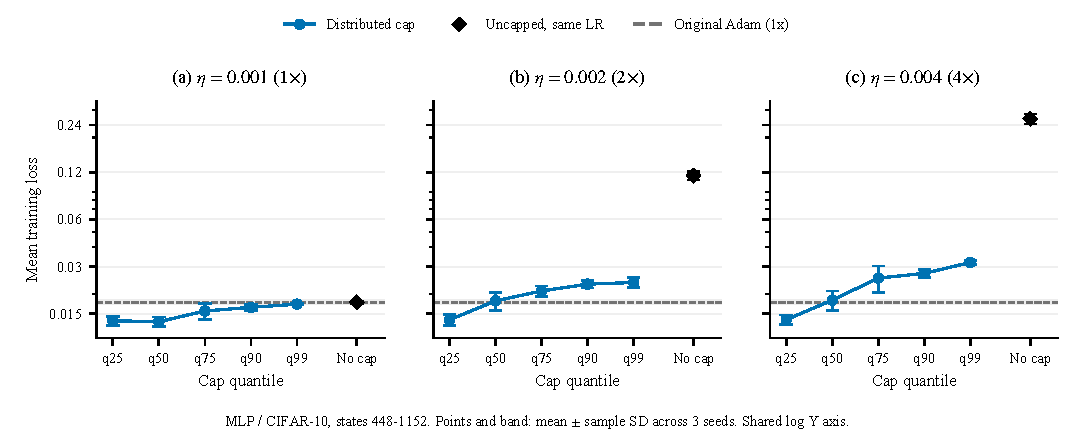
\includegraphics[width=7.15in]{figures/14-distributed-cap-quantile-ablation-mlp.pdf}
\caption{Historical MLP quantile-by-rate ablation across three initializations, with each treated branch compared with its same-rate unchanged-Adam control and with original Adam. Budgets are calibrated at the original rate and fixed across multipliers. The historical 448--1152 window differs from the main 512--800 MLP comparison. Increasing nominal rate does not improve mean training loss over the same cap at the original rate. The plotted uncertainty is sample variation across three initializations, not update-level replication.}
\end{figure}

\clearpage
\section{Reproducibility and Scope of the Evidence}

The companion reproduction package retains the publication PDFs, editable equations and algorithms, compact numerical tables, figure manifests, and their source observations. Generating scripts specify each transformation, smoothing rule, clock conversion, and coverage restriction. Experiment inputs and retrieved artifacts have recorded SHA-256 identities; native replay, numerical reductions, and observer checks precede figure construction. The reported comparisons use frozen scientific configurations, with historical and matched-grid measurements kept separate.

\begin{table}[H]
\centering\small
\caption{Evidence provenance by scientific question. Identifiers locate the versioned source observations in the reproduction package, rather than denoting additional independent experiments.}
\begin{tabular}{@{}lp{4.9in}@{}}
\toprule
Question & Source scope \\
\midrule
GD curvature and accumulation & Analysis 024 (nine trajectories and loss residuals), 035 (backward lags), 056 (all-pair and endpoint audit) \\
Sampling and independent HVPs & Analyses 027/037; three initialization blocks, frozen-state controls, and matched moving continuations \\
Adam severity and timing & Analysis 055; nine original full-objective Adam arms, complete decisions and horizon/memory reductions \\
Functional tracing & Analyses 062/063; reference-set event windows, with the revised ResNet fit from Run 292 \\
Matched interventions & Analysis 065, Runs 293--295; 36 common-state conditions with full post-treatment coverage \\
Historical MLP sensitivity & Analysis 065, Runs 286--288; 54 continuations with separate windows and calibration \\
\bottomrule
\end{tabular}
\end{table}

The main paper distinguishes exact identities, smooth approximations, empirical associations, and controlled treatment effects. Observed counts are not all independent: updates and windows overlap, stages share a network, and settings share one initialization. The sampling study's three initializations and historical MLP replication do not supply missing independent initializations for the main Adam grid. Likewise, single reference sets and selected event windows establish participation and temporal structure without identifying unique causes or spike-specific modes.

Initializations 1/2 for the complete matched intervention matrix, the cross-model cap-by-rate grid, quiet-window and contrasts across reference sets, and prospective forecasting remain additional experiments. None is represented as completed here. The present evidence supports the bounded conclusions in the main paper; stronger reliability, causal, generalization, or computational-efficiency claims require their corresponding tests.

\clearpage
\section{Extended Intervention Trajectories}
\label{supp:extended-interventions}
Figures~\ref{fig:app-updates}--\ref{fig:app-selected} retain complete
post-intervention update histories, intervention activity, and selected
representation trajectories. The applied increments differ from raw
gradients; nominal coefficients do not match effective intervention
strength. The selected conventional settings illustrate contrasting
behaviors, rather than rank each family's best setting. Section S5
retains the complete matched outcomes.

\begin{figure}[H]
\centering
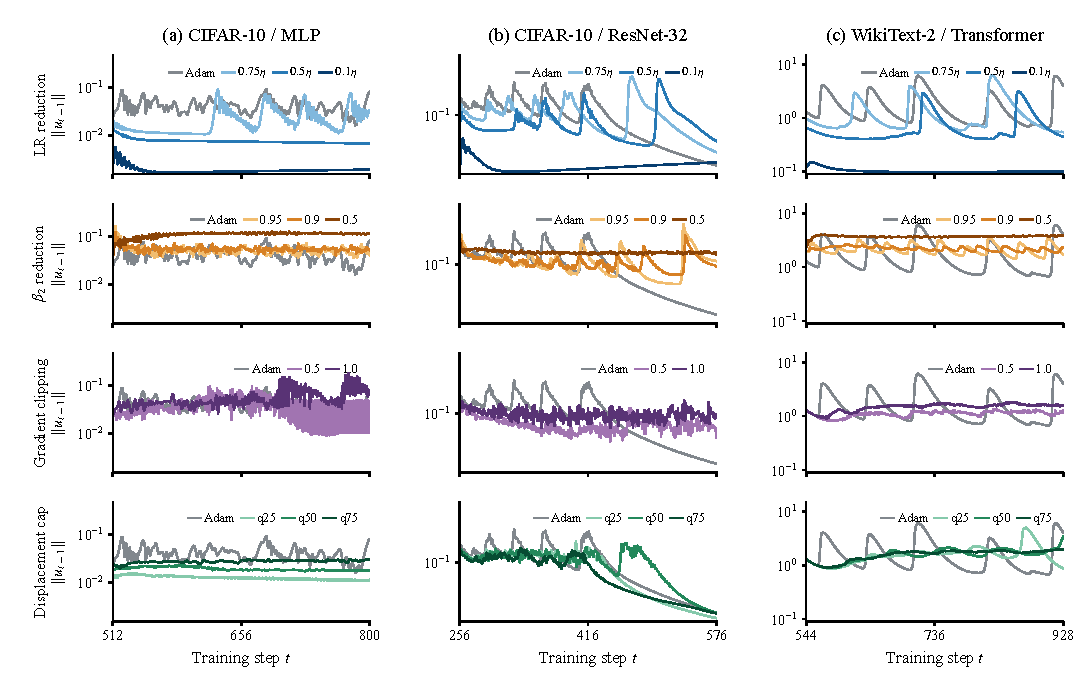
\includegraphics[width=\linewidth,height=.78\textheight,keepaspectratio]{figures/a01-matched-applied-updates.pdf}
\caption{Actual applied update norms for all matched interventions. Rows correspond to immediate learning-rate reduction, late $\beta_2$ reduction, global gradient clipping, and distributed displacement caps. Gray is the same unchanged-Adam control in every row. All post-start updates are retained without smoothing; the log scale is shared across families within each model. Update $u_{t-1}$ is placed at its completed-state endpoint $t$.}
\label{fig:app-updates}
\end{figure}

\clearpage
\begin{figure}[H]
\centering
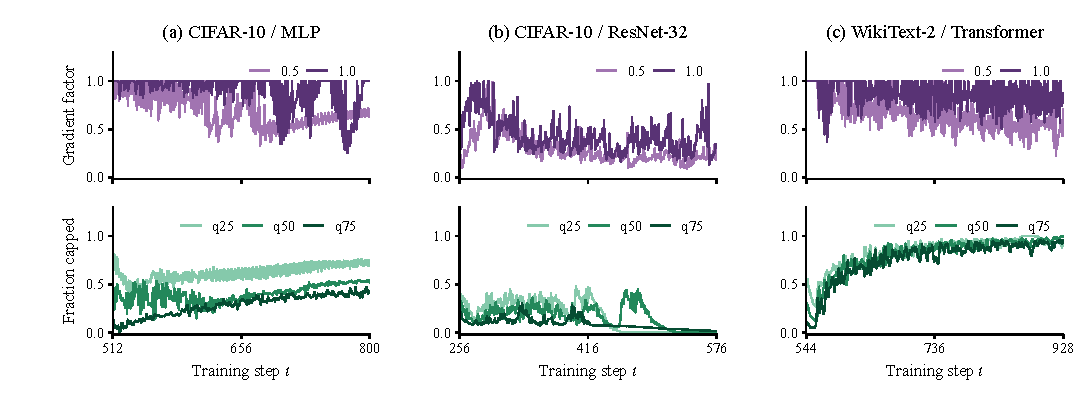
\includegraphics[width=\linewidth,height=.78\textheight,keepaspectratio]{figures/a02-matched-controller-activity.pdf}
\caption{Controller activity over the same complete windows. Top: multiplicative factor retained by global gradient clipping before Adam; one means no clipping. Bottom: fraction of targeted units whose proposed increments are scaled by the displacement cap, pooled over all targeted sites; zero means no units capped. A clipping factor is not an Adam update-retention factor. All values are aligned with completed updates and unsmoothed.}
\label{fig:app-activity}
\end{figure}

\clearpage
\begin{figure}[H]
\centering
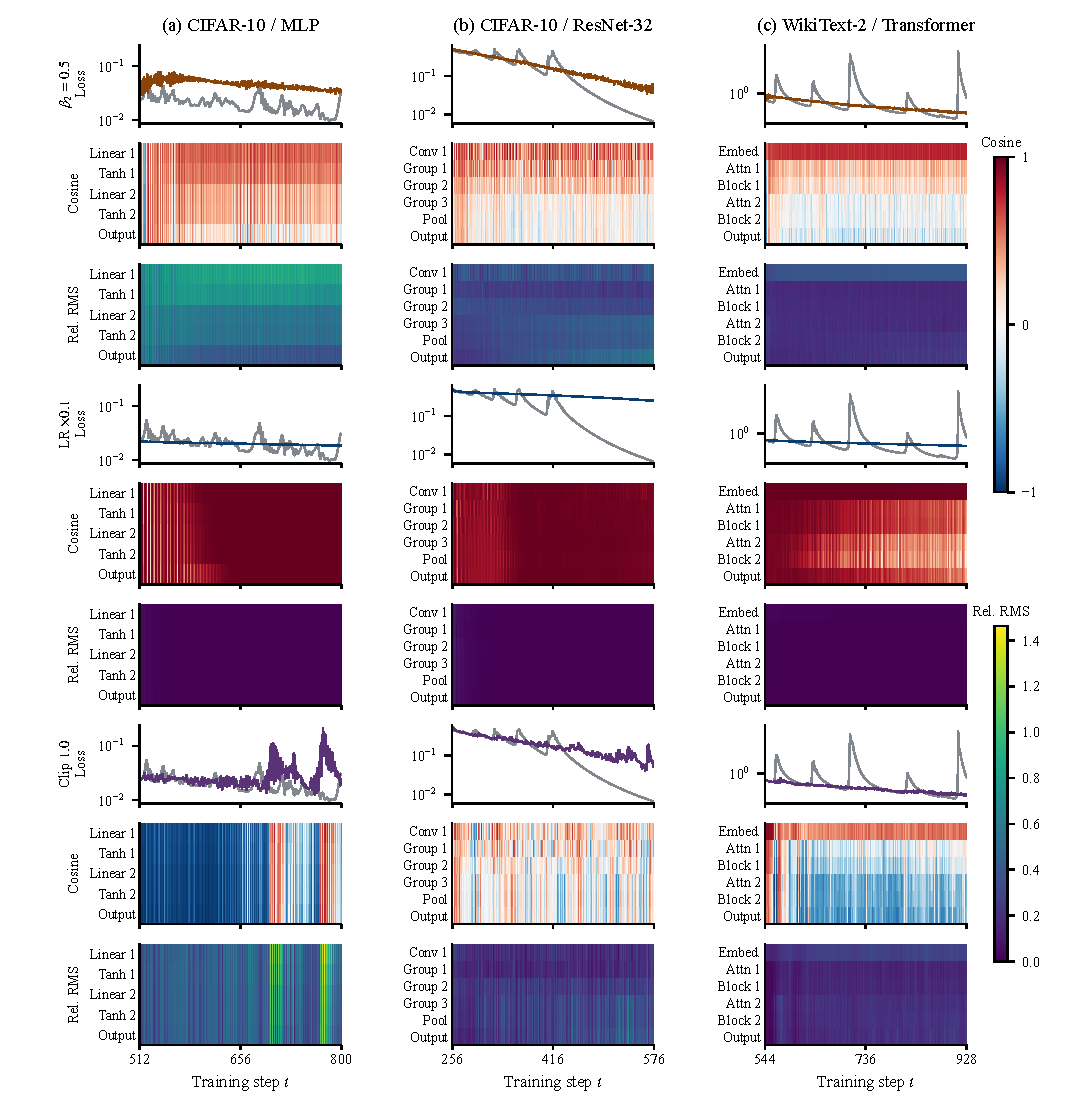
\includegraphics[width=\linewidth,height=.78\textheight,keepaspectratio]{figures/a03-selected-intervention-motion.pdf}
\caption{Selected conventional interventions across the three models: $\beta_2=0.5$ (top block), LR $\times0.1$ (middle), and clip threshold 1.0 (bottom). Each block shows full training loss, consecutive representation-change cosine, and relative RMS displacement. Gray loss curves are unchanged Adam; colored curves and all heatmaps belong to the selected intervention. No Adam heatmaps are repeated. Log-loss limits are shared across the three blocks within each model. RMS uses each site's unchanged-Adam maximum as a common denominator, with one color scale across all selected settings and models; values above one exceed that baseline maximum. Every post-start change is retained, without smoothing, layer averaging, or peak markers. Sites match the main paper's representation-motion figure.}
\label{fig:app-selected}
\end{figure}
\clearpage

\bibliographystyle{IEEEtran}
\bibliography{references}
\end{document}
